%
% Documento: Apêndice
%

\begin{apendicesenv}
\partapendices

\renewcommand{\figurename}{Figura A.}
\renewcommand{\tablename}{Tabela A.}
\setcounter{figure}{0}
\setcounter{table}{0}

\section*{Apêndice A: \textit{Stellar Parameter Estimation and Calculation Tools for Research and Analysis} (SPECTRA)}\label{ap:spectra}

Como uma maneira de otimizar a determinação de massa para dferentes aglomerados, construiu-se o \textit{software} \textit{Stellar Parameter Estimation and Calculation Tools for Research and Analysis} (SPECTRA),que encontra-se atualmente em sua versão de 2024.12.15t, e foi desenvolvido por João Paulo Matos Dias Gomes, disponível em \url{https://github.com/Gomes-JP/spectra}. Trata-se de uma ferramenta versátil projetada para a análise e cálculo de propriedades estelares, incluindo massa, idade, luminosidade, temperatura, raio e distância. O \textit{software} integra funcionalidades como ajuste de isócronas, modelagem por regressão, imputação de dados e visualização. Ele depende de bibliotecas Python amplamente utilizadas, como \texttt{numpy}, \texttt{pandas} e \texttt{ttkbootstrap}, garantindo compatibilidade com fluxos de trabalho astrofísicos estabelecidos.

A principal motivação para o desenvolvimento do SPECTRA é a necessidade de ferramentas acessíveis, precisas e abrangentes para pesquisas astrofísicas. O \textit{software} atende a essa demanda oferecendo uma interface amigável (Figura A.1) e algoritmos avançados para análise do comportamento estelar. Ele permite que pesquisadores e educadores estimem parâmetros estelares chave, modelem estados evolutivos e visualizem dados de forma eficaz.


 \begin{figure}[!h]
	\centering
	\caption[Interface gráfica do \textit{software} SPECTRA.] {Interface gráfica desenvolvida para as ferramentas do \textit{software} SPECTRA.}
	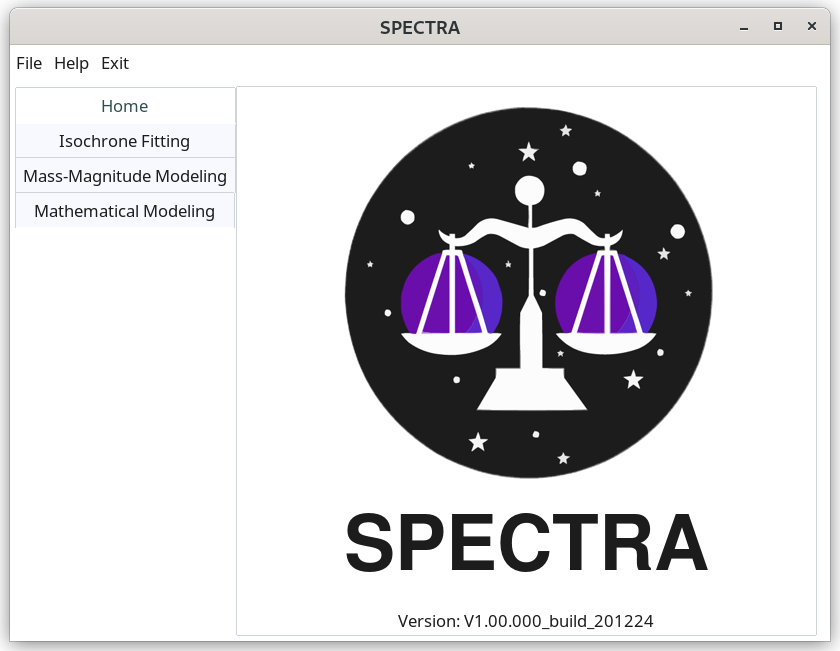
\includegraphics[width=0.7\linewidth]{04-figuras/interface_a}
	\label{fig:interface}
\end{figure}

O \textit{software} processa dados fornecidos no formato CSV, utilizando consultas estruturadas para extrair e analisar parâmetros estelares a partir de dados de modelos teóricos de evolução e interior estelar. Ele inclui funcionalidades para filtrar conjuntos de dados e lidar com entradas incompletas, implementar métodos de imputação como KNN e técnicas iterativas para tratar dados ausentes, além de mapear propriedades estelares observadas em isócronas teóricas. Essas capacidades garantem que os dados de entrada sejam preparados e processados de forma eficaz, permitindo a geração de modelos confiáveis e precisos.

A inspeção de dados é parte integrante do fluxo de trabalho do SPECTRA. Os usuários podem explorar seus conjuntos de dados de forma interativa por meio de ferramentas visuais, como diagramas HR e gráficos de diagnóstico, que ajudam a interpretar relações complexas entre estrelas. O \textit{software} também permite que os usuários realizem análises de correlação para identificar as características mais relevantes para os parâmetros alvo. Além disso, relatórios de desempenho resumem a precisão dos modelos utilizando métricas como RMSE, MAE e R² (Tabela \ref{tab:model_performance}), permitindo aos usuários avaliar e refinar suas análises.

\begin{table}[htbp]
	\centering
	\caption[Relatório estatístico de modelagem]{Exemplo de relatório das métricas obtidas para os modelos gerados para o melhor conjunto de Hiperparâmetros de cada algoritmo.}
	\label{tab:model_performance}
	\begin{tabular}{lccccc}
		\hline
		\textbf{Modelo} & \textbf{RMSE} & \textbf{MAE} & \textbf{R²} & \textbf{AIC} & \textbf{Score} \\
		\hline
		Bayesian & 0.077 & 0.067 & 0.942 & -511.024 & 0.997 \\
		Linear & 0.077 & 0.067 & 0.942 & -511.026 & 0.997 \\
		ElasticNet & 0.077 & 0.068 & 0.942 & -510.409 & 1.000 \\
		Support Vector & 0.006 & 0.006 & 1.000 & -988.982 & 0.104 \\
		Decision Tree & 0.002 & 0.002 & 1.000 & -1243.508 & 0.041 \\
		Random Forest & 0.001 & 0.001 & 1.000 & -1400.027 & 0.018 \\
		Gradient Boosting & 0.001 & 0.001 & 1.000 & -1437.803 & 0.013 \\
		AdaBoost & 0.008 & 0.007 & 0.999 & -943.724 & 0.123 \\
		KNeighbors & 0.000 & 0.000 & 1.000 & -1560.472 & 0.000 \\
		\hline
	\end{tabular}
\end{table}




O SPECTRA possui planos para desenvolvimento contínuo, visando, além da melhora na sua funcionalidade, a integração de novos módulos com novas funções. Atualizações futuras incluirão a integração de modelos teóricos de evolução e interior estelar adicionais, ampliando a gama de dados suportados. O \textit{software} também contará com a otimização automatizada para modelos de regressão e ajuste de isócronas, reduzindo o esforço manual. O desenvolvimento de APIs permitirá a integração com outras ferramentas e bases de dados astrofísicas, aumentando sua versatilidade.

\end{apendicesenv}